\documentclass{pack}

\begin{document}

    \title{Amplificadores de Potência tipo \emph{push-pull}}
    \author{Bianca Yoshie Itiroko - 164923, Luiz Eduardo Cartolano - 183012, Seong Eun Kim - 177143 \\ EE534 - Turma Y - Grupo 2}
    \date{Outubro de 2018}
    
    \maketitle
    
    \begin{abstract}
        Esse experimento teve como objetivo construir um estágio de potência com a topologia \emph{push-pull} e estudar sua eficiência, comparando com o estágio de acoplamento montado no experimento anterior. Através dele, pudemos obter a potência de $1,9KW$ o seguidor de emissor, de $0W$ para o \emph{push-pull} simples com alimentação assimétrica e $8W$ para o \emph{push-pull} com polarização e alimentação assimétrica. Assim, podemos concluir que o primeiro tem uma potência maior em relação aos demais.
    \end{abstract}
    
    \section{Introdução}
        O transístor de junção bipolar, \emph{BJT}, é o tipo de transístor mais comum presente no mercado, devido a sua facilidade de polarização e durabilidade. Seu nome se dá fruto do seu processo de condução, que é realizado por dois tipos de carga - positiva (lacunas) e negativa (elétrons).  São normalmente compostos de três terminais, sendo os eles, a Base, o Emissor(\emph{Emitter}) e o Coletor(\emph{Collector}). Existem essencialmente dois tipos de \emph{BJT}, o do tipo NPN e PNP. Os transístores \emph{BJT} tem uma série de aplicações práticas no nosso dia a dia, sendo especialmente usados como amplificadores de corrente(ou tensão) e como controle \emph{ON-OFF}(chaves do tipo liga-desliga).
    
        Um dos circuitos mais usados com a aplicação de transistores \emph{BJT} são os circuitos \emph{push-pull}. Um amplificador como este é um tipo de circuito eletrônico que usa um par de dispositivos ativos que, alternadamente, fornecem corrente ou absorvem corrente de uma carga conectada. Um amplificador desse tipo é mais eficiente que um amplificador "classe A" de terminação única, por isso seu uso é menos custoso e de grande interesse para quem precisa utilizá-lo. 
    
        Neste experimento será estudado o comportamento do circuito \emph{push-pull}, desde sua configuração mais simples (vide Figura \ref{fig:pushSimp}) até implementações bem mais complexas, como a da Figura \ref{fig:pushPol}. Também estudaremos seu uso em conjunto com circuitos pré-amplificadores e junto a caixas alto-falante e microfones de eletreto.
    
    \section{Procedimentos}
        Para a realização dos experimentos propostos, foram utilizados os seguintes componentes e ferramentas: Osciloscópio digital de dois canais, gerador de ondas/funções, fonte de tensão contínua, cabos com plugs banana e coaxial, multímetro digital, placa de contatos, transístores \emph{BSS100 ,2N2222 e 2N2907}, um resistor de potência de $56\Omega (5W)$, capacitores de $220nF$, $680nF$ e $1\mu F$ resistores de $82\Omega$, $2,2k\Omega$ e $6,8k\Omega$, e diodos \emph{1N4004}. Além de um alto-falante e um microfone de eletreto.
    
        A primeira parte consiste na familiarização dos alunos com o novo circuito estudado, para isso montou-se o circuito que pode ser observado na Figura \ref{fig:pushSimp}, com $C1 = 680nF$ e $C2 = 220uF$. Nesta etapa buscou-se analisar o funcionamento básico dos transistores e a saída encontrada. Um detalhe importante para essa etapa é, além do cuidado especial com a polarização do transistor é limitar a corrente emitida pela fonte de tensão contínua em $200mA$.
        
        Na segunda etapa do laboratório, buscou-se estudar configurações mais complexas do circuito \emph{push-pull}. Primeiro, substituímos a alimentação que antes era simétrica por uma alimentação assimétrica, como podemos ver na Figura \ref{fig:pushAssi}, para o circuito também foram adicionados dois resistores de $2,2K\Omega$. Por fim, montou-se um circuito ainda mais complexo, que pode ser visto na Figura \ref{fig:pushPol}. Este, recebe um acréscimo de dois diodos do tipo 1N4004, cujas funções serão melhor discutidas na Seção \ref{sec:discussao}. Novamente, devemos ressaltar a importância de se atentar a polarização dos transistores (especialmente agora que transistores \emph{NPN} e \emph{PNP} serão usados em conjunto). Além disso, deve-se manter o limitador de corrente na fonte de tensão contínua, a fim de garantir a segurança do circuito.
        
        Por fim, vale ressaltar que as análise mencionadas para o circuito simplificado serão refeitas nos demais circuitos. É interessante notar também que o resistor de carga destes circuitos (\emph{$R_L$}) será a caixa alto-falante.

    \section{Discussão} \label{sec:discussao}
        Para o circuito seguidor de emissor, aterrou-se a entrada do circuito e mediu-se a ddp em $R_E$, que foi de $11,15V$. Como $R_E$ tem resistência de $82\Omega$, a corrente era de $136mA$. Calculou-se a tensão em $V_{BE}$, de $0,7V$, o que foi acima do esperado ($0,6V$), o que indica que a tensão alta em $R_E$ se deve a corrente alta.
        
        Para o estágio \textit{push-pull}, com a entrada e saída desconectadas, mediu-se $V_B = 1mV$ e $V_E = 8,6mV$ (ou seja, tensão desprezível). Isso está dentro do esperado pois a ddp nos transistores é menor do que o limiar, de forma que eles não conduzem.
        
        Ao aplicar-se na entrada uma onda triangular de tensão de $200mV_{pp}$ e frequência de $1kHz$, observou-se que na saída houve deformação da onda de entrada, como pode ser visto na Figura \ref{fig:newFile5}. Aumentando-se gradualmente a tensão de entrada, observou-se que a deformação e a amplitude diminuiu. Com $400mV_{pp}$, a onda observada está na Figura \ref{fig:newFile6}.
        
        Depois, ligou-se uma carga na saída (caixa de som) e repetiu-se o procedimento anterior. Observou-se bastante distorção na onda de saída, como pode ser visto na Figura \ref{fig:newFile4}. Isso se é esperado pois a caixa de saída tende a deformar a onda de saída vista no osciloscópio já que há conversão das ondas elétricas em sonoras que são por ela transmitidas.
        
        Em seguida, montou-se o circuito da Figura \ref{fig:pushSimp}. Os resistores desse circuito são responsáveis pela polarização dos transistores, garantindo uma menor distorção do sinal de saída. A polarização acontece pois a corrente ao passar pelo resistor gera uma queda de tensão. O circuito no entanto ainda não é perfeito, se os ruídos não existissem na Figura \ref{fig:newFile7} seria possível observar uma região na qual os dois transistores estão desligados, este problema será corrigido com a inserção dos diodos, como veremos a seguir.
        
        Aterrou-se a entrada e mediu-se a tensão sobre a carga $R_L$. Obteve-se aproximadamente $0V$. Pela fórmula \ref{eq:ganho_tensao}, pode-se concluir que a potência dissipada é nula. Adicionando uma onda triangular ao circuito foi possível observar que começa a existir circulação de corrente nele. A partir de uma entrada de $700mV_{pp}$ os transistores são ativados, como observado na Figura \ref{fig:newFile7}, além disso, com uma caixa de som conectada, é possível ouvir sons a partir desse valor. Um problema encontrado no sinal de saída observado é a distorção deste e os "bicos" presentes, provavelmente eles são fruto de interferência causada pelo capacitor nos seus ciclos de carga e descarga.
        
        Em seguida, aplicou-se uma forma de onda triangular de $200mV_{pp}$ e frequência de $1KHz$. Nessa configuração, não houve ruído na caixa de som. Então, aumentou-se gradativamente o sinal de entrada e, com aproximadamente $720mV_{pp}$, começou-se a ouvir ruídos. Pode-se observar a onda de saída na Figura \ref{fig:newFile7}. Vê-se que a onda de saída, que deveria ser triangular, possui bastante deformação, tanto na subida, como na descida. Também é possível notar uma grande quantidade de ruído, causada pelo mau contato dos componentes do circuito.
        
        Para a próxima parte do experimento, adicionou-se dois diodos ao circuito do push-pull. Os mesmos tem como função polarizar ambos os transistores no corte, garantindo uma tensão entre a base e o emissor entre $0,6$ e $0,7V$ de forma que a distorção no cruzamento se sobrepõe e o efeito pode ser minimizado.
        
        Com a entrada aterrada, foi então possível medir $V_{BE} = 0,608V$, $V_{R1} = 4,18V$ e $V_{R2} = 3,6V$, de modo que foi possível calcular $I_{R1} = 1,9mA$, $I_{R2} = 1,63mA$, $I_{B1} = I_{B2} = 0,13mA$ e $I_{C} = 0,54mA$. Então, com o auxílio de um amperímetro ligado em série no circuito, calculou-se a potência total dissipada no circuito com o diodo, que foi cerca de $8W$. Voltando ao circuitos vistos no início da atividade, é possível perceber uma ganho considerável quando comparado ao seguidor de emissor, que gastava uma potência em torno de $1,9KW$, justificando o uso do circuito \emph{push-pull}. A potência para o circuito \emph{push-pull} sem o diodo foi, para nós, de 0W, pois infelizmente não calculamos a corrente sobre os resistores, a fim de ter valores mais precisos. A análise dessas potências nos mostra o motivo pelo qual o circuito com diodos deve ser adotado, já que, além de gastar pouquíssima energia, ele não deforma a onda de saída e nem tem momentos no qual ambos os transistores estão em corte.
        
        Aplicando uma forma de onda triangular de $200mV_{PP}$ e $1KHz$. Ainda sem carga, mediu-se o ganho de tensão correspondente e observou-se a distorção no circuito pela \ref{fig:newFile8}. Assim, buscando avaliar o comportamento do mesmo, variou-se a frequência para $4Hz$ e observou-se a Figura \ref{fig:newFile9}.
        
        Ao comparar ambas, pode-se notar que a medida que aumentamos a frequência, pode-se notar que há uma diminuição na distorção gerada, de forma que com amplificação maior, a onda de saída começa a se assemelhar em forma à da entrada.
        
        Acoplando uma carga a saída, pode-se observar a Figura \ref{fig:newFile10} e ao tentar realizar uma avaliação acerca do aumento da frequência, obteve-se a Figura \ref{fig:newFile11}. Pode-se observar que ao aumentar-se a frequência, aumentou também os ruídos advindos da adição da carga, de forma que pode-se inferir que houve sim um ganho de tensão, mas de valor não confiável, devido a alta oscilação do mesmo.
        
        A última parte do experimento não pode-se ser realizada pois não houve tempo hábil.
        
    \section{Conclusão}
    Neste experimento buscou-se analisar a eficiência dos estágios construídos para um amplificador de carga. Ao testar o circuito seguidor de emissor do experimento anterior, houve uma grande deformação da onda de entrada que, a medida que a tensão aumentava, a deformação e a amplitude diminuíam.
    
    Para o circuito \emph{push-pull simples}, ouviu-se o sinal de entrada na caixa de som conectada a partir de $720mV_{pp}$, a uma frequência de $1kHz$. Porém, no sinal de saída houve uma grande distorção e "bicos" presentes, que representavam a interferência do capacitor em seus ciclos de carga e descarga e o mau funcionamento dos cabos.
    
    Para a última parte do experimento, a medida que aumentou-se a frequência, a distorção diminui e então a onda de saída começa a se assemelhar a de entrada. Ao conectarmos a carga, como nos demais circuitos do experimento, as distorções aumentaram consideravelmente, assim como os ruídos. Pode-se inferir que houve ganho de tensão, apesar do valor não ser confiável devido a alta oscilação.
    
    Dentre esses três circuitos, o que obteve maior potência foi o primeiro, com valor de $1,9KW$.
    
    
    \nocite{*}
    \bibliographystyle{plain}
    \bibliography{references}
    
    \newpage
    \section*{ANEXOS}
    %%%%%%%%%%%%%%%%%
    %   EQUAÇÕES    %
    %%%%%%%%%%%%%%%%%

    \begin{eqfloat}[h!]
        \begin{equation}
            P = I * R^{2}
            \label{eq:ganho_tensao}
        \end{equation}
        \caption{Fórmula da potência dissipada por uma carga.}
    \end{eqfloat}
    
    
    %%%%%%%%%%%%%%%
    %   FIGURAS   %
    %%%%%%%%%%%%%%%
    \begin{figure}[h!]
        \centering
        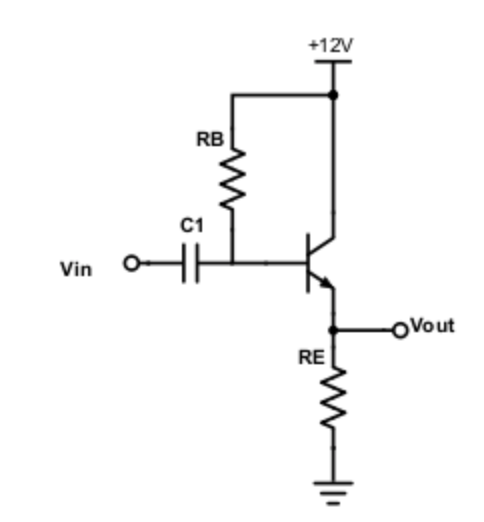
\includegraphics[height=5.5cm]{imgSource/circuitolab4.png}
        \caption{Circuito seguidor de emissor com transístor BJT.}
        \label{fig:circLab4}
    \end{figure}
    
    \begin{figure}[h!]
        \centering
        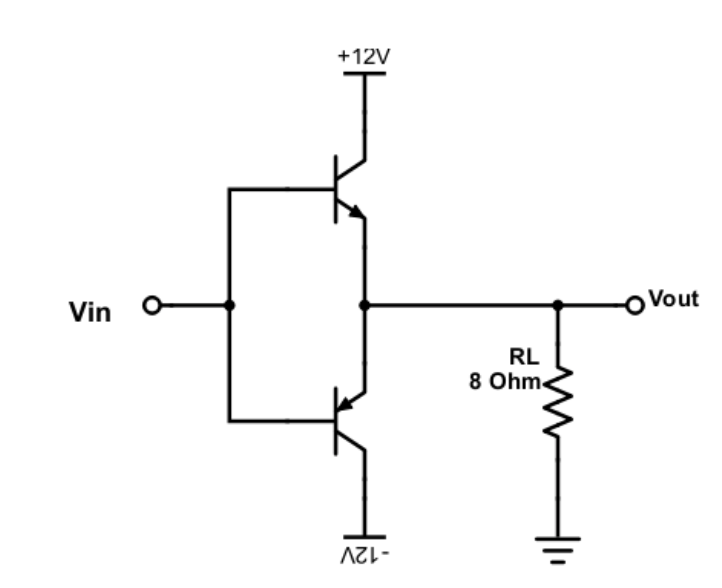
\includegraphics[height=5.5cm]{imgSource/pushPullSimp.png}
        \caption{Circuito \emph{push-pull} simples.}
        \label{fig:pushSimp}
    \end{figure}
    
    \begin{figure}[h!]
        \centering
        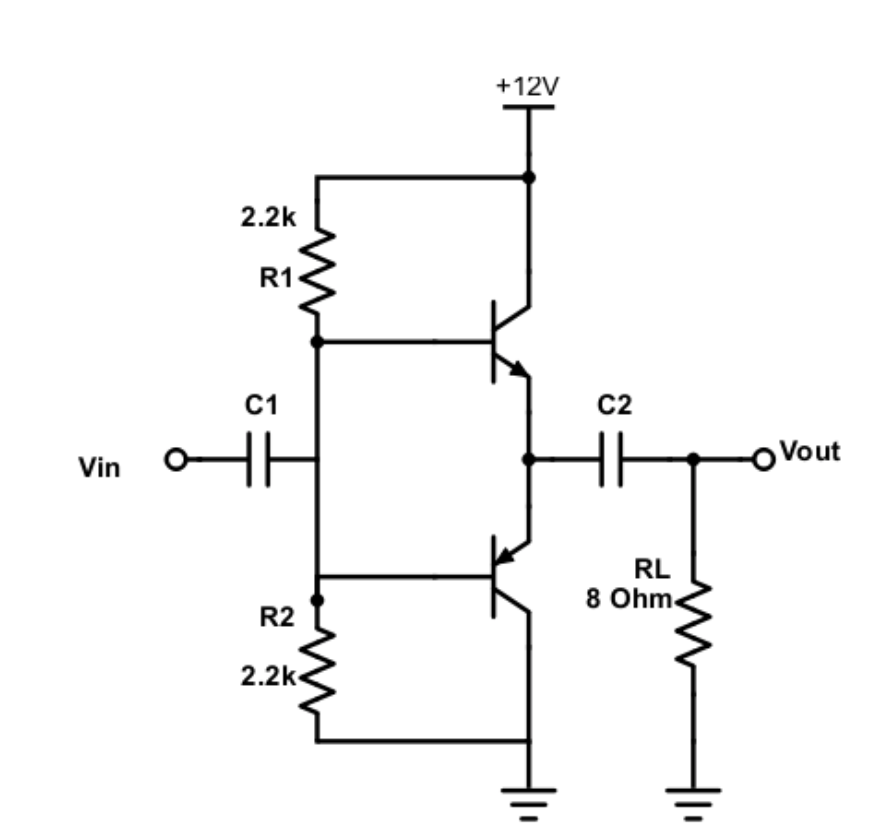
\includegraphics[height=5.5cm]{imgSource/pushPullAssi.png}
        \caption{Circuito \emph{push-pull} simples com alimentação assimétrica.}
        \label{fig:pushAssi}
    \end{figure}
    
    \begin{figure}[h!]
        \centering
        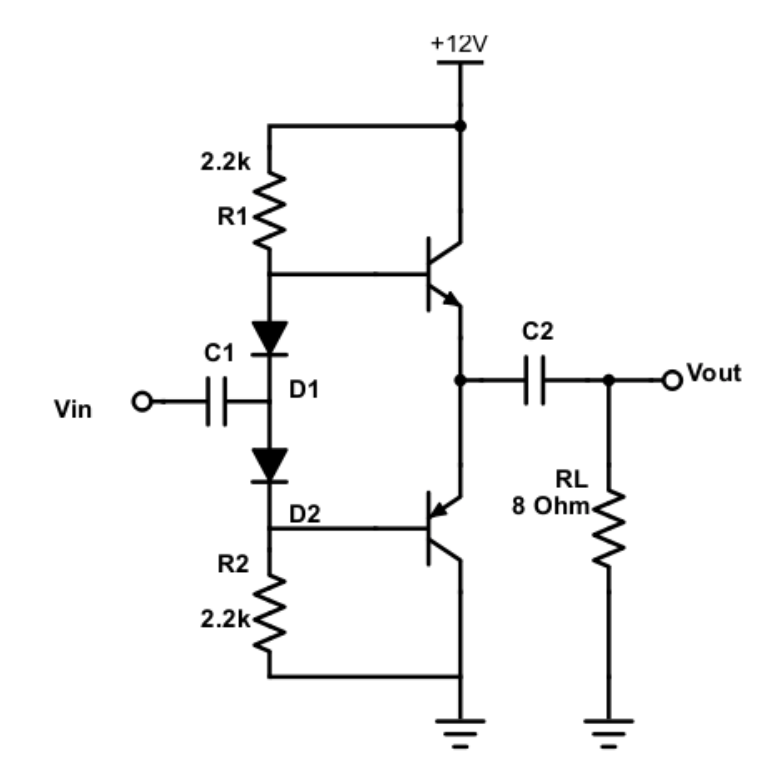
\includegraphics[height=5.5cm]{imgSource/pushPullPol.png}
        \caption{Circuito \emph{push-pull} com polarização e alimentação assimétrica.}
        \label{fig:pushPol}
    \end{figure}
    
    \begin{figure}[h!]
        \centering
        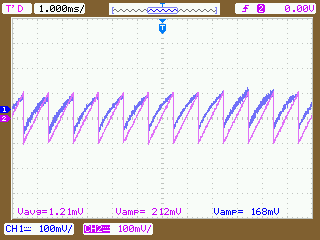
\includegraphics[height=5.5cm]{imgSource/oscilloscope/NewFile0.png}
        \caption{Sinal de saída do circuito push-pull com deformação.}
        \label{fig:newFile0}
    \end{figure}
    
    \begin{figure}[h!]
        \centering
        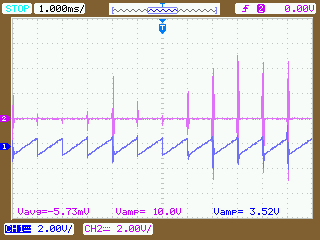
\includegraphics[height=5.5cm]{imgSource/oscilloscope/NewFile4.png}
        \caption{Sinal de saída com a carga (alto-falante) acoplada.}
        \label{fig:newFile4}
    \end{figure}
    
    \begin{figure}[h!]
        \centering
        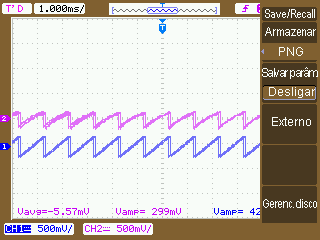
\includegraphics[height=5.5cm]{imgSource/oscilloscope/NewFile5.png}
        \caption{Sinal de saída para sinal de entrada de $200mV_{PP}$.}
        \label{fig:newFile5}
    \end{figure}
    
    \begin{figure}[h!]
        \centering
        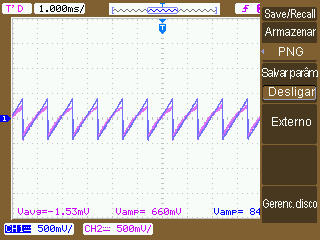
\includegraphics[height=5.5cm]{imgSource/oscilloscope/NewFile6.png}
        \caption{Sinal de saída para sinal de entrada de $400mV_{PP}$.}
        \label{fig:newFile6}
    \end{figure}
    
    \begin{figure}[h!]
        \centering
        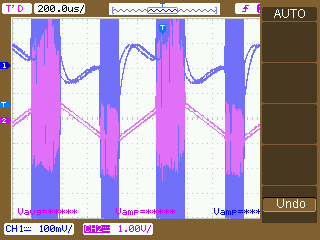
\includegraphics[height=5.5cm]{imgSource/oscilloscope/NewFile7.png}
        \caption{Sinal de saída para o circuito push-pull com entrada assimétrica.}
        \label{fig:newFile7}
    \end{figure}
    
    \begin{figure}[h!]
        \centering
        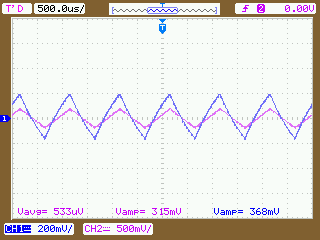
\includegraphics[height=5.5cm]{imgSource/oscilloscope/NewFile8.png}
        \caption{Sinal de saída para o circuito com diodos e entrada de 1KHz.}
        \label{fig:newFile8}
    \end{figure}
    
    \begin{figure}[h!]
        \centering
        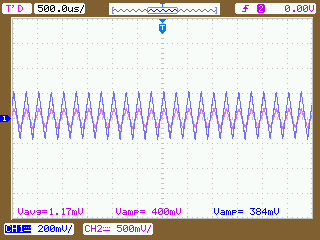
\includegraphics[height=5.5cm]{imgSource/oscilloscope/NewFile9.png}
        \caption{Sinal de saída para o circuito com diodos e entrada de 4KHz.}
        \label{fig:newFile9}
    \end{figure}
    
    \begin{figure}[h!]
        \centering
        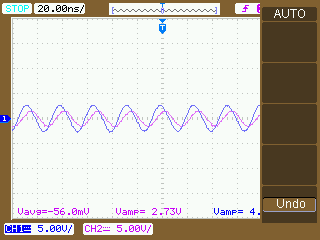
\includegraphics[height=5.5cm]{imgSource/oscilloscope/NewFile10.png}
        \caption{Sinal de saída para o circuito com diodos e entrada de 1KHz e carga (alto-falante acoplado.}
        \label{fig:newFile10}
    \end{figure}
    
    \begin{figure}[h!]
        \centering
        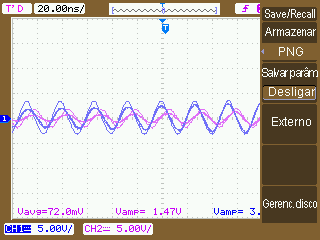
\includegraphics[height=5.5cm]{imgSource/oscilloscope/NewFile11.png}
        \caption{Sinal de saída para o circuito com diodos e entrada de 4KHz e carga (alto-falante acoplado.}
        \label{fig:newFile11}
    \end{figure}
    
    
    

\end{document}